\documentclass[xcolor=svgnames]{beamer}

%-=-=-=-=-=-=-=-=-=-=-=-=-=-=-=-=-=-=-=-=-=-=-=-=
% LOADING BASIC PACKAGES
%-=-=-=-=-=-=-=-=-=-=-=-=-=-=-=-=-=-=-=-=-=-=-=-=

\usepackage[utf8]{inputenc}
\usepackage[T1]{fontenc}
\usepackage[english] {babel}
\usepackage{amsmath,amsfonts,graphicx}
\usepackage{beamerleanprogress}
\usepackage{pstricks}

%-=-=-=-=-=-=-=-=-=-=-=-=-=-=-=-=-=-=-=-=-=-=-=-=
%        LOADING TIKZ LIBRARIES
%-=-=-=-=-=-=-=-=-=-=-=-=-=-=-=-=-=-=-=-=-=-=-=-=

\usetikzlibrary{
backgrounds,
mindmap,
shapes.arrows,
positioning,
}

\tikzset{
    myarrow/.style={
        draw,
        fill=orange,
        single arrow,
        minimum height=7.5ex,
        single arrow head extend=1ex
    }
}
\newcommand{\arrowup}{%
\tikz [baseline=-0.5ex]{\node [myarrow,rotate=90] {};}
}
\newcommand{\arrowdown}{%
\tikz [baseline=2ex]{\node [myarrow,rotate=-90] {};}
}

\tikzstyle{every picture}+=[remember picture]
\tikzstyle{na} = [baseline=-.5ex]

%-=-=-=-=-=-=-=-=-=-=-=-=-=-=-=-=-=-=-=-=-=-=-=-=
% LOADING EXTRA PACKAGES
%-=-=-=-=-=-=-=-=-=-=-=-=-=-=-=-=-=-=-=-=-=-=-=-=

%\usepackage[colorlinks=false, urlcolor=blue, pdfborder={0 0 0}]{hyperref} 
\usepackage{chngcntr}
\usepackage{float}
%\usepackage{titlepic}
\usepackage{array}
\usepackage{multirow}
\usepackage{booktabs}
\usepackage{dcolumn}
\usepackage{bibentry}
\usepackage{wasysym, marvosym}


%-=-=-=-=-=-=-=-=-=-=-=-=-=-=-=-=-=-=-=-=-=-=-=-=
% SMART TABLES
%-=-=-=-=-=-=-=-=-=-=-=-=-=-=-=-=-=-=-=-=-=-=-=-=

\setlength{\heavyrulewidth}{0.1 em}
\newcommand{\otoprule}{\midrule [\heavyrulewidth]}
\usepackage[small,bf]{caption}
%\captionsetup[table,figure]{labelfont=bf,font=small}
%%%%%%%%%%%%%%%%%%%%%%%%%%%%%%%%%%%%%%%%%%%%%%%%%%%%%%%%%%%%%%%%%%%%%%%%%%%%%%%%%%%%%%%%%%

%-=-=-=-=-=-=-=-=-=-=-=-=-=-=-=-=-=-=-=-=-=-=-=-=
% NUMBERING CAPTIONS
%-=-=-=-=-=-=-=-=-=-=-=-=-=-=-=-=-=-=-=-=-=-=-=-=
\setbeamertemplate{caption}[numbered]

%-=-=-=-=-=-=-=-=-=-=-=-=-=-=-=-=-=-=-=-=-=-=-=-==-=-=-=-=
% REMOVAL OF DEFAULT SYMBOL BIBLIOGRAPHY IN BEAMER CLASS
%-=-=-=-=-=-=-=-=-=-=-=-=-=-=-=-=-=-=-=-=-=-=-=-==-=-=-=-=
\setbeamertemplate{bibliography item}[text]

%-=-=-=-=-=-=-=-=-=-=-=-=-=-=-=-=-=-=-=-=-=-=-=-=
% INSERTING TEXT INSIDE BOXES
%-=-=-=-=-=-=-=-=-=-=-=-=-=-=-=-=-=-=-=-=-=-=-=-=
\setbeamercolor{postit}{bg=yellow!70!green}

%-=-=-=-=-=-=-=-=-=-=-=-=-=-=-=-=-=-=-=-=-=-=-=-=
% TO USE ACCENT IN "I" in Spanish
%-=-=-=-=-=-=-=-=-=-=-=-=-=-=-=-=-=-=-=-=-=-=-=-=
\newcommand{\1}{\'{\i}}

%-=-=-=-=-=-=-=-=-=-=-=-=-=-=-=-=-=-=-=-=-=-=-=-=
% TITLE PAGE
%-=-=-=-=-=-=-=-=-=-=-=-=-=-=-=-=-=-=-=-=-=-=-=-=

\title
  [Feb 2016 \hspace{3cm} Krakow]
  {General Introduction to Radioactivity}
  
\author
  [J.L. Guti\'errez--Villanueva]
  {Jos\'e - Luis Guti\'errez Villanueva}

\date
  {February 2016}

\institute
  {LaRUC,  University of Cantabria (Spain)}

\titlegraphic{
\includegraphics[scale=0.25]{laruc_logo}	}


%-=-=-=-=-=-=-=-=-=-=-=-=-=-=-=-=-=-=-=-=-=-=-=-=
% DOCUMENT
%-=-=-=-=-=-=-=-=-=-=-=-=-=-=-=-=-=-=-=-=-=-=-=-=

\begin{document}

\maketitle

%-=-=-=-=-=-=-=-=-=-=-=-=-=-=-=-=-=-=-=-=-=-=-=-=
%
%	TABLE OF CONTENTS: OVERVIEW
%
%-=-=-=-=-=-=-=-=-=-=-=-=-=-=-=-=-=-=-=-=-=-=-=-=

\section*{Overview}
\begin{frame}{}
% For longer presentations hideallsubsections
\tableofcontents[hideallsubsections]
\end{frame}

%\section{Introduction}

%\frame{\tableofcontents[currentsection]}

\begin{frame}{Once upon a time \ldots}

\begin{columns}[T]

    \begin{column}{.5\textwidth}
    
\begin{minipage}[c][.6\textheight][c]{\linewidth}
\begin{figure}
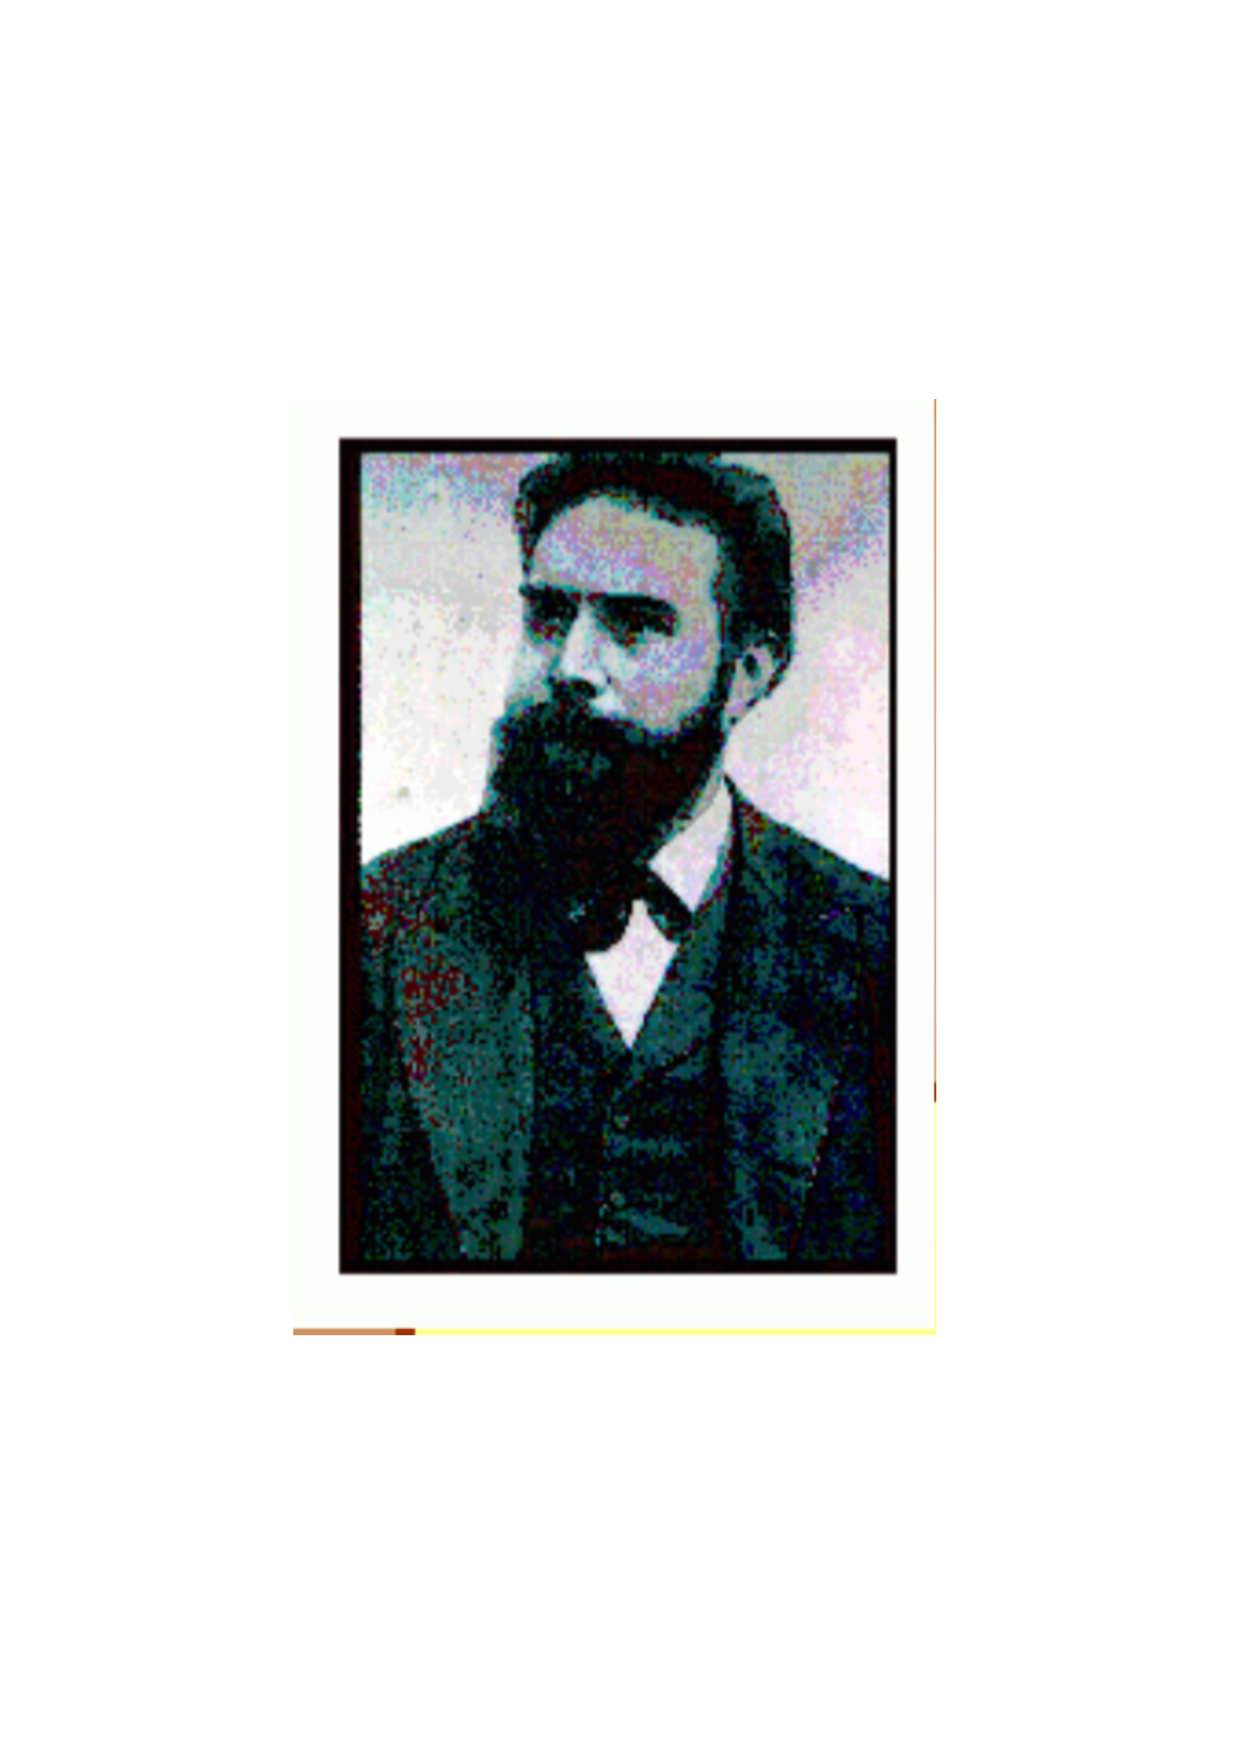
\includegraphics[scale=0.3]{figures/roentgen.pdf}
\end{figure}    
\end{minipage}    
    
 
    \end{column}
    
    \begin{column}{.5\textwidth}
    
\begin{minipage}[c][.6\textheight][c]{\linewidth}
            \begin{itemize}
                \item X- rays
\item Some materials emit radiation 
\item Wow ! we can penetrate our body
            \end{itemize}
          \end{minipage}    
    
    
    \end{column}
    
    
\end{columns}




\end{frame}

\begin{frame}{Once upon a time \ldots}

\begin{figure}
\vskip-4cm
\centering
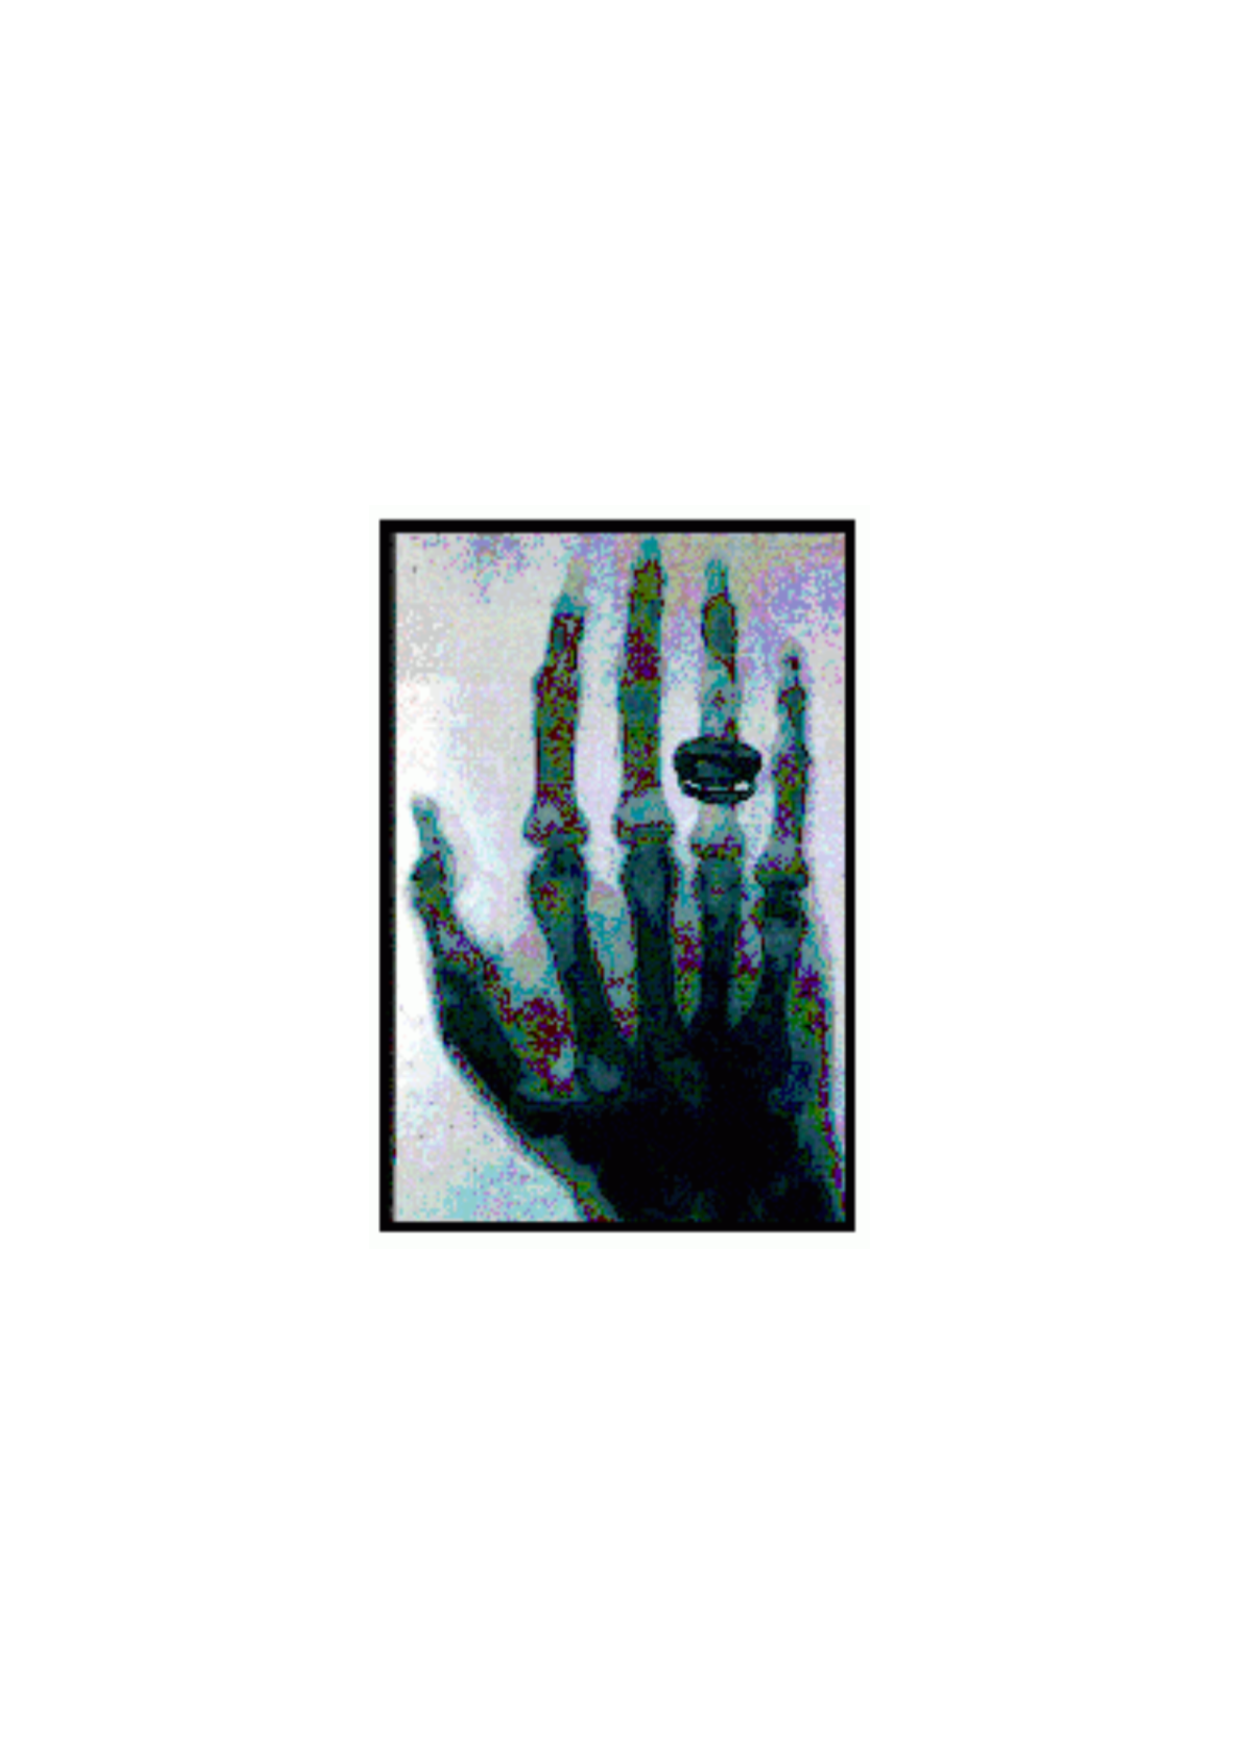
\includegraphics[scale=0.5]{figures/20160216_rsw_roentgenhand.pdf}
\end{figure}
\end{frame}

\begin{frame}{Once upon a time \ldots}

\begin{columns}[T]

    \begin{column}{.5\textwidth}
    
\begin{minipage}[c][.6\textheight][c]{\linewidth}
\begin{figure}
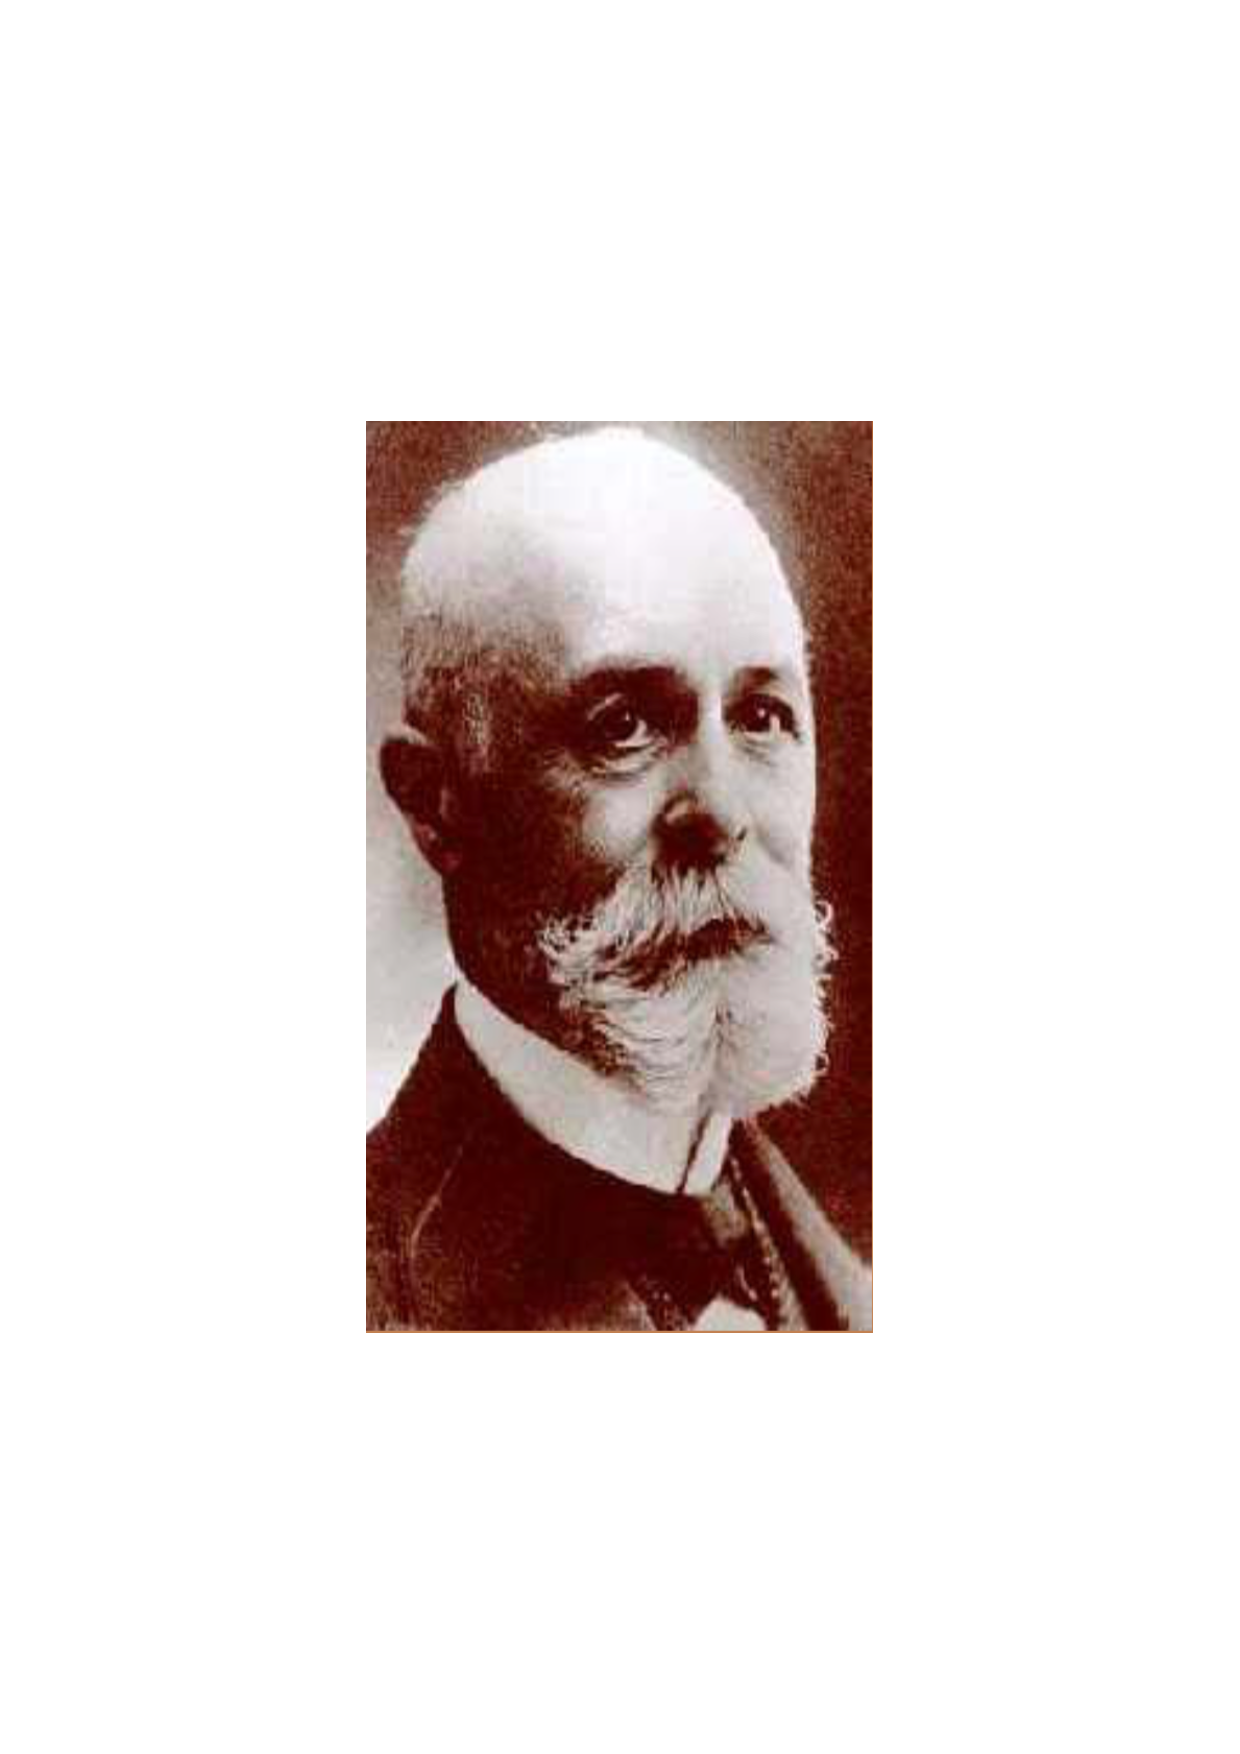
\includegraphics[scale=0.3]{figures/20160216_rsw_becquerel.pdf}
\end{figure}    
\end{minipage}    
    
 
    \end{column}
    
    \begin{column}{.5\textwidth}
    
\begin{minipage}[c][.6\textheight][c]{\linewidth}
            \begin{itemize}
               \item Photographic plates can get dark in the presence of material called Uranium
\item It must a property of the matter itself
\item Such a material emits a type of radiation	
            \end{itemize}
          \end{minipage}    
    
    
    \end{column}
    
    
\end{columns}


\end{frame}


\begin{frame}{Once upon a time \ldots}

\centering MARIE SKLODOWSKA and PIERRE CURIE

\vskip-1cm
\begin{columns}[T]

    \begin{column}{.35\textwidth}
     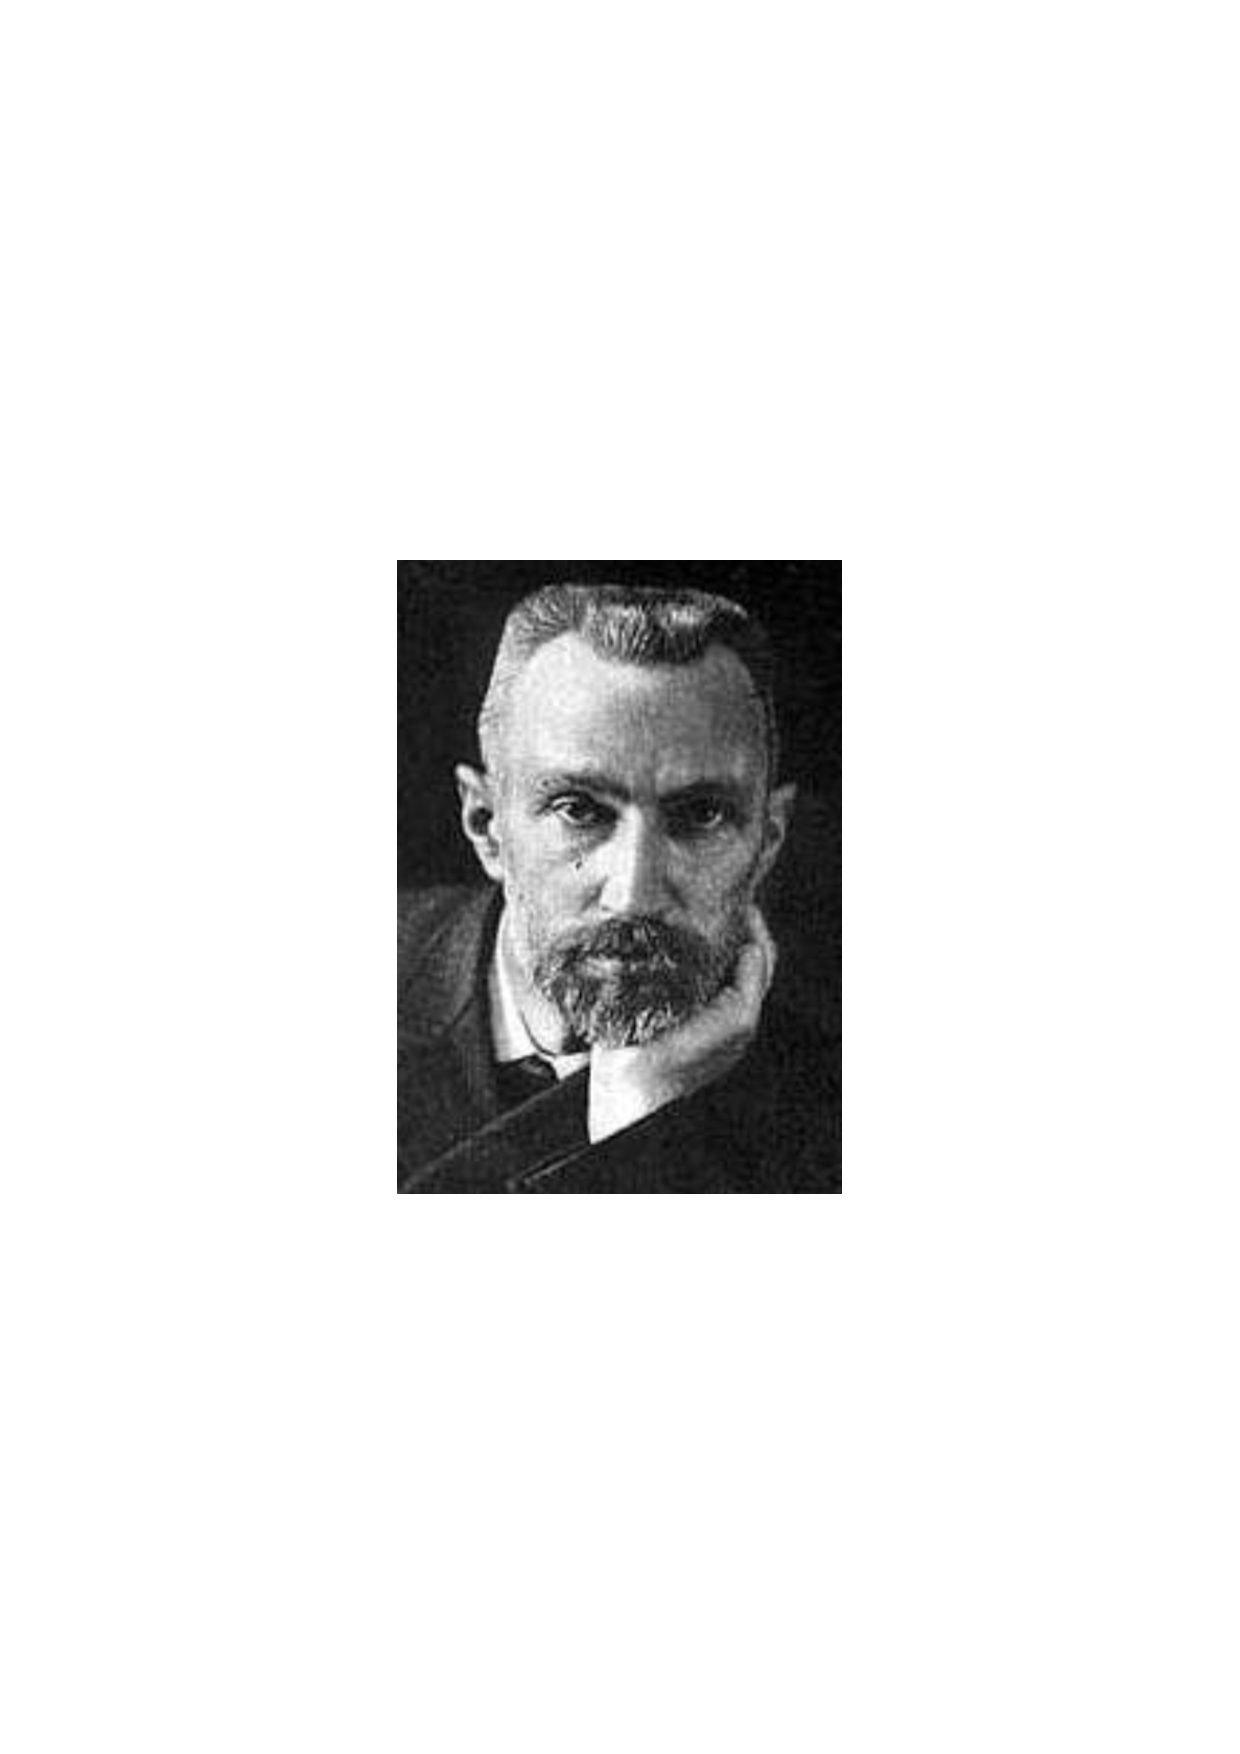
\includegraphics[scale=0.3]{figures/20160216_rsw_pierrecurie.pdf}
    \end{column}
    
    \begin{column}{.3\textwidth}
    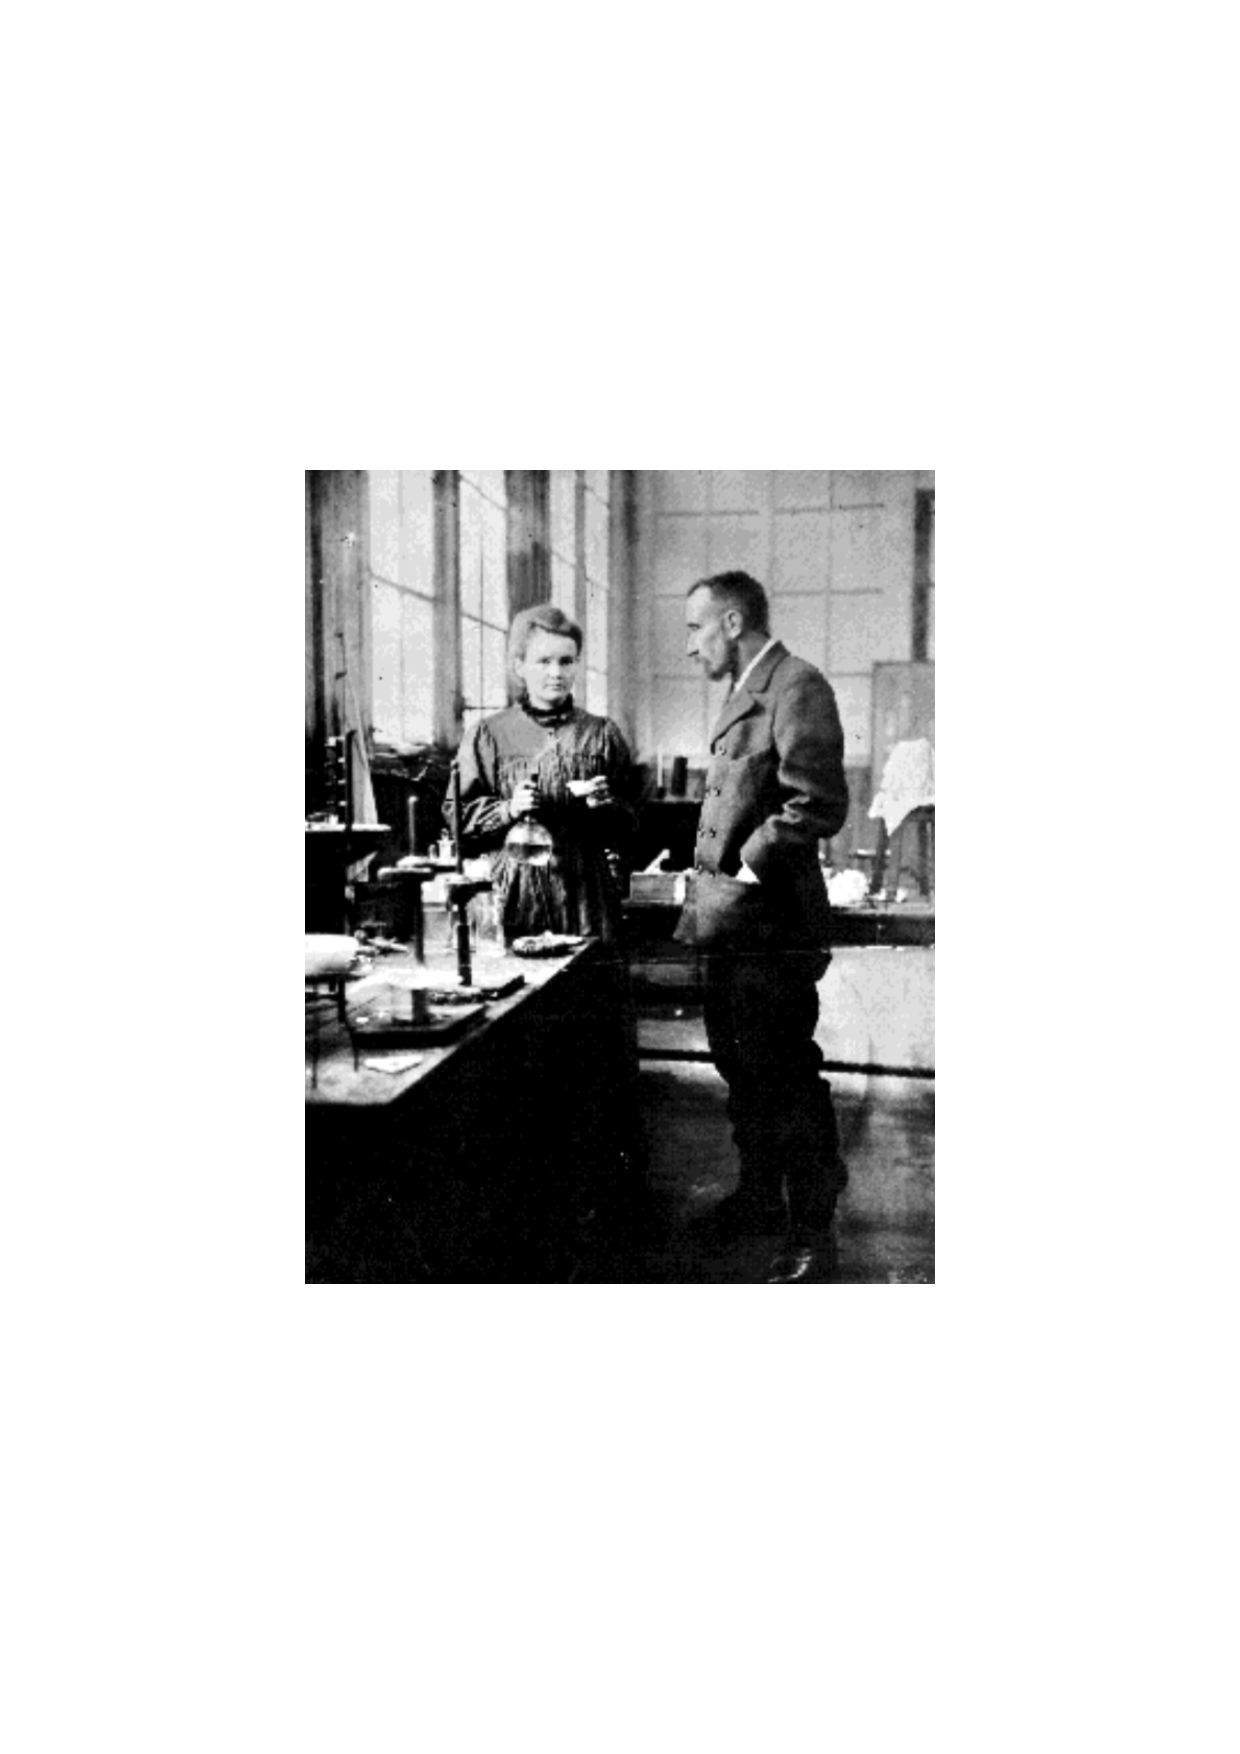
\includegraphics[scale=0.25]{figures/20160216_rsw_mariepiere.pdf}
    \end{column}
    
    \begin{column}{.6\textwidth}
   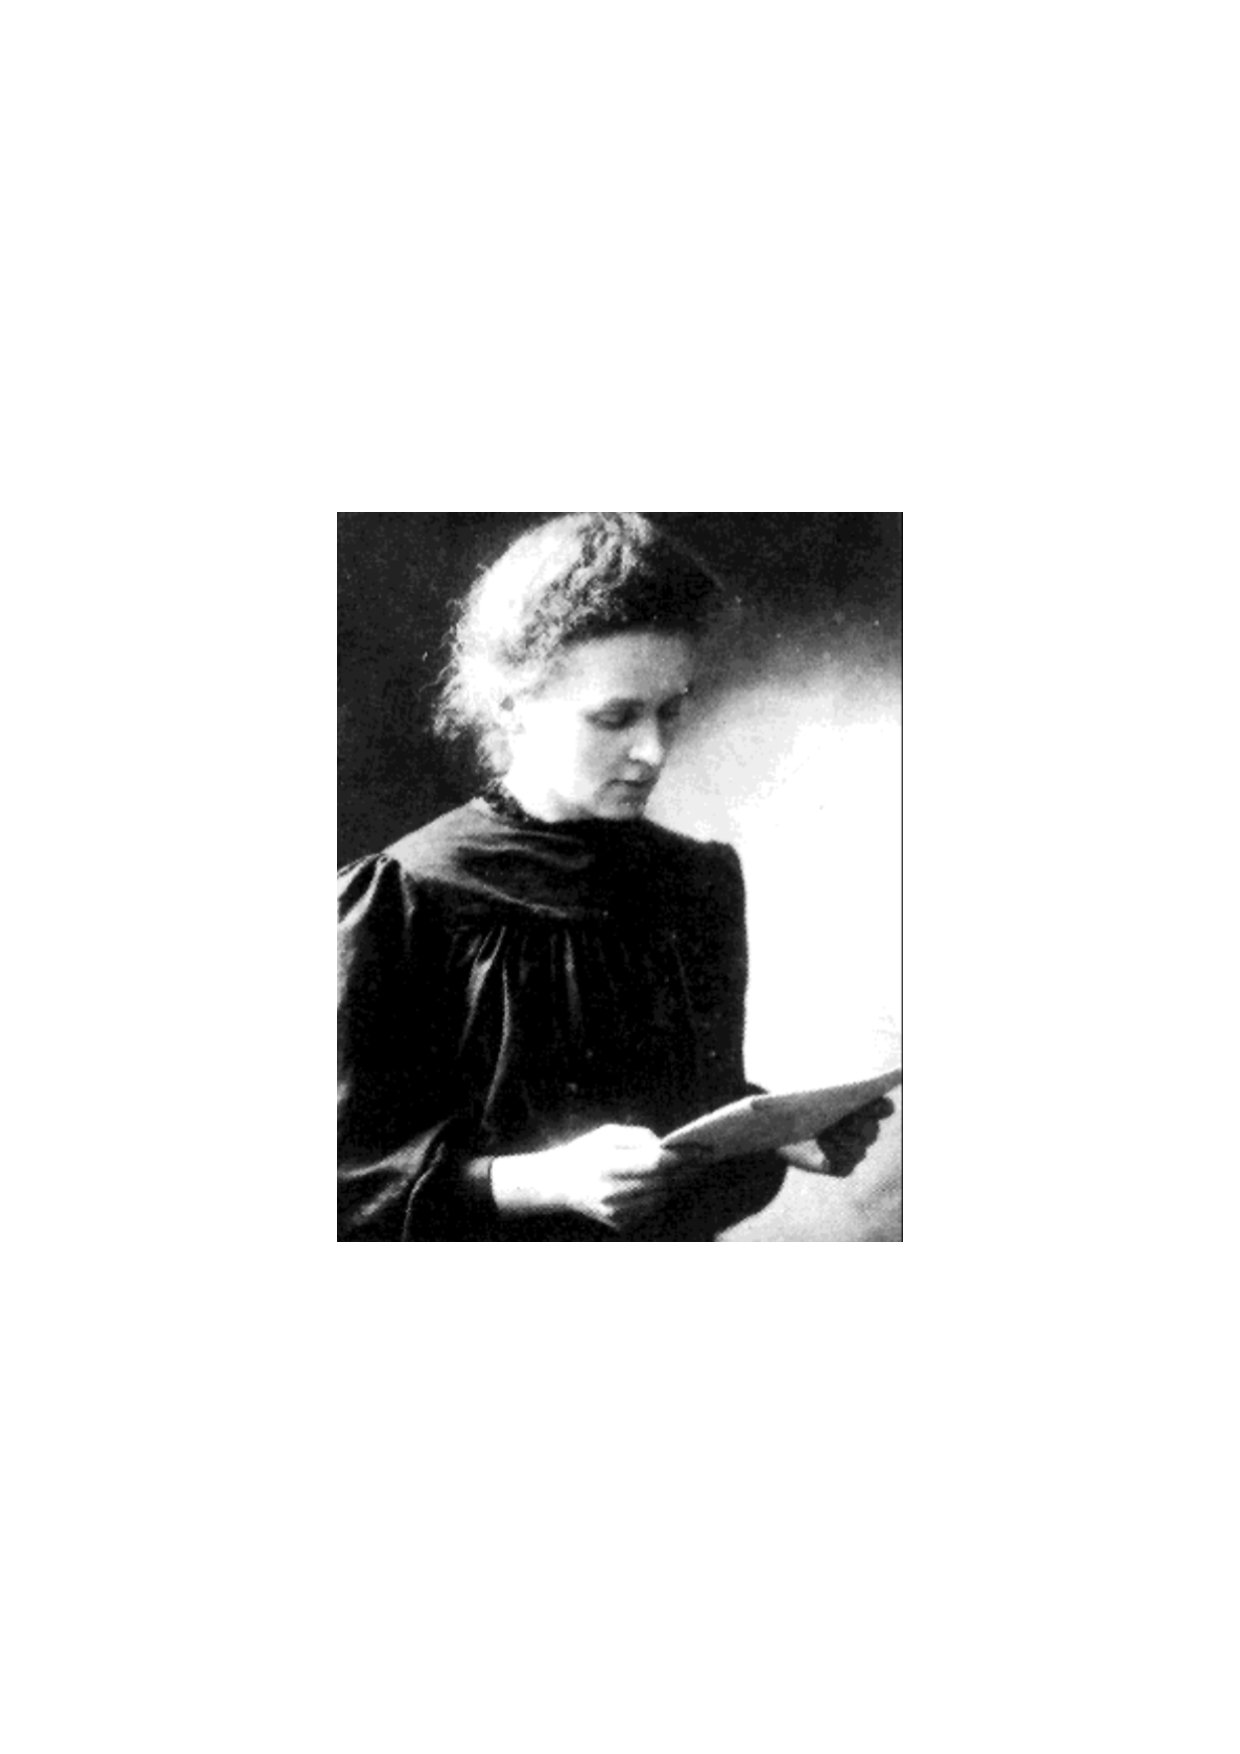
\includegraphics[scale=0.3]{figures/20160216_rsw_marie.pdf}
    \end{column}

\end{columns}

\end{frame}

\begin{frame}{Once upon a time \ldots}

  \begin{exampleblock}{A wonderful marriage}
   \begin{itemize}
   \item Marie: a physicist and mathematician but \ldots a Polish Woman
   \item Pierre: professor of Physics in Paris
   \item Studies on pitchblende 
   \end{itemize}
  \end{exampleblock}

\vskip-4cm
\centering 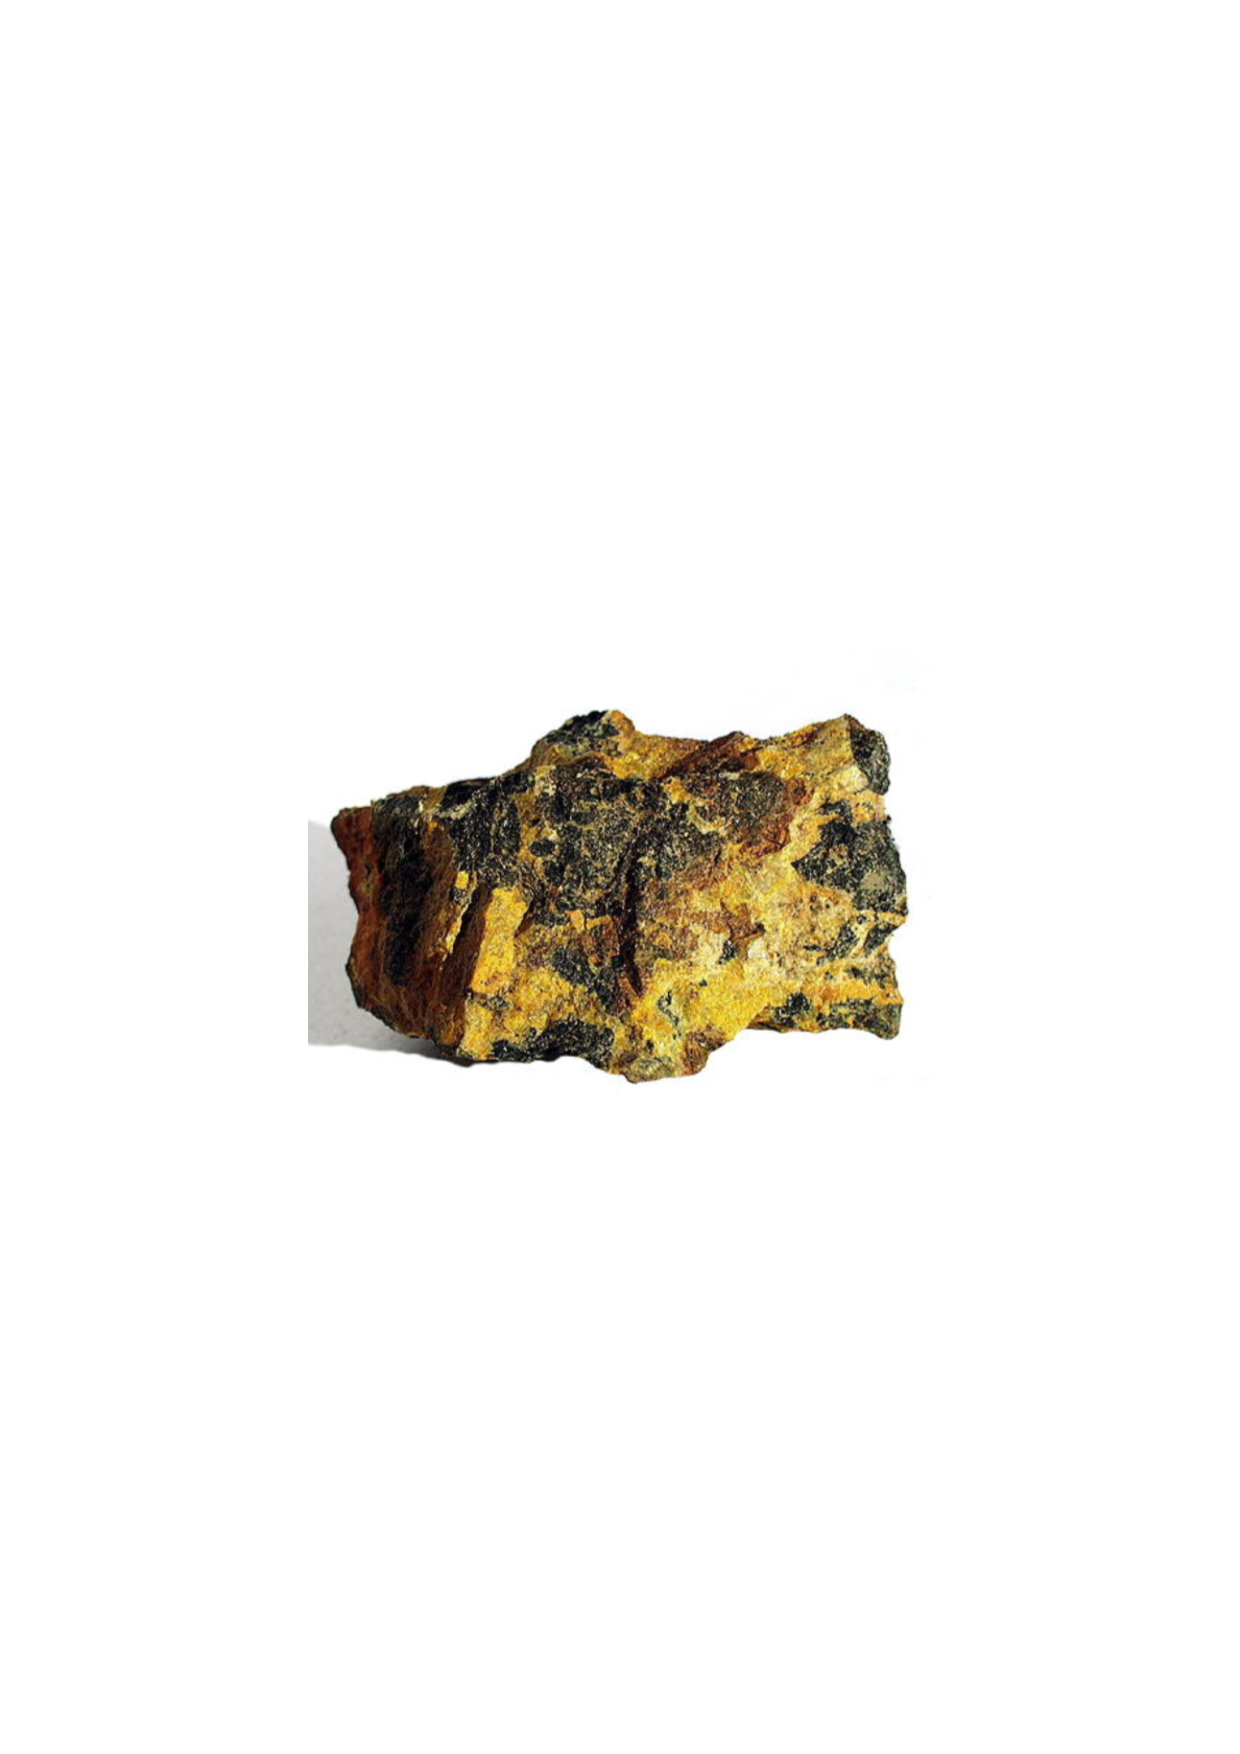
\includegraphics[scale=0.4]{figures/20160216_rsw_pechblenda.pdf}

\end{frame}

\begin{frame}{Once upon a time \ldots}

\begin{exampleblock}{Their work with pitchblende}

\begin{itemize}

\item They began separating elements and reducing sample's size
\item They observe an increase on the intensity of emitted radiation
\item They discovered \textbf{Polonium} in 1898

\end{itemize}

\end{exampleblock}

\end{frame}

\begin{frame}{Once upon a time \ldots}

\begin{exampleblock}{Their work with pitchblende}

\begin{itemize}

\item After separation of Plonium \ldots emitted radiation increases more and more
\item It must be another element different from Uranium and different from Radium. This element emits radiation too.
\pause \item \ldots the Radium 
\item It is necessary to determine its chemical and physical properties

\pause \begin{itemize}
\item Very poor materials and infraestructures to do the task
\item Laboratory: a simple shed
\item From pitchblende to radium: years and years of hard work
\pause \item $10^3$kg pitchblende $\Longrightarrow$ few grams of radium
\end{itemize}

\end{itemize}

\end{exampleblock}

\end{frame}

\begin{frame}{Once upon a time \ldots}

\begin{exampleblock}{Milestones}

\begin{itemize}
\item 1903: Nobel prize on Physics: Marie, Pierre and Becquerel (15000 \$ !!!)
\item 1906: Pierre Curie passed away in a street accident in Paris on 19 April 1906 ({\footnotesize\textit{Crossing the busy Rue Dauphine in the rain at the Quai de Conti, he slipped and fell under a heavy horse-drawn cart. He died instantly when one of the wheels ran over his head, fracturing his skull (\emph{Wikipedia})}})
\item 1911: Nobel prize on Chemistry: Marie Curie
\end{itemize}

\end{exampleblock}

\end{frame}

\begin{frame}{Once upon a time \ldots}
\vskip-3.5cm
\centering
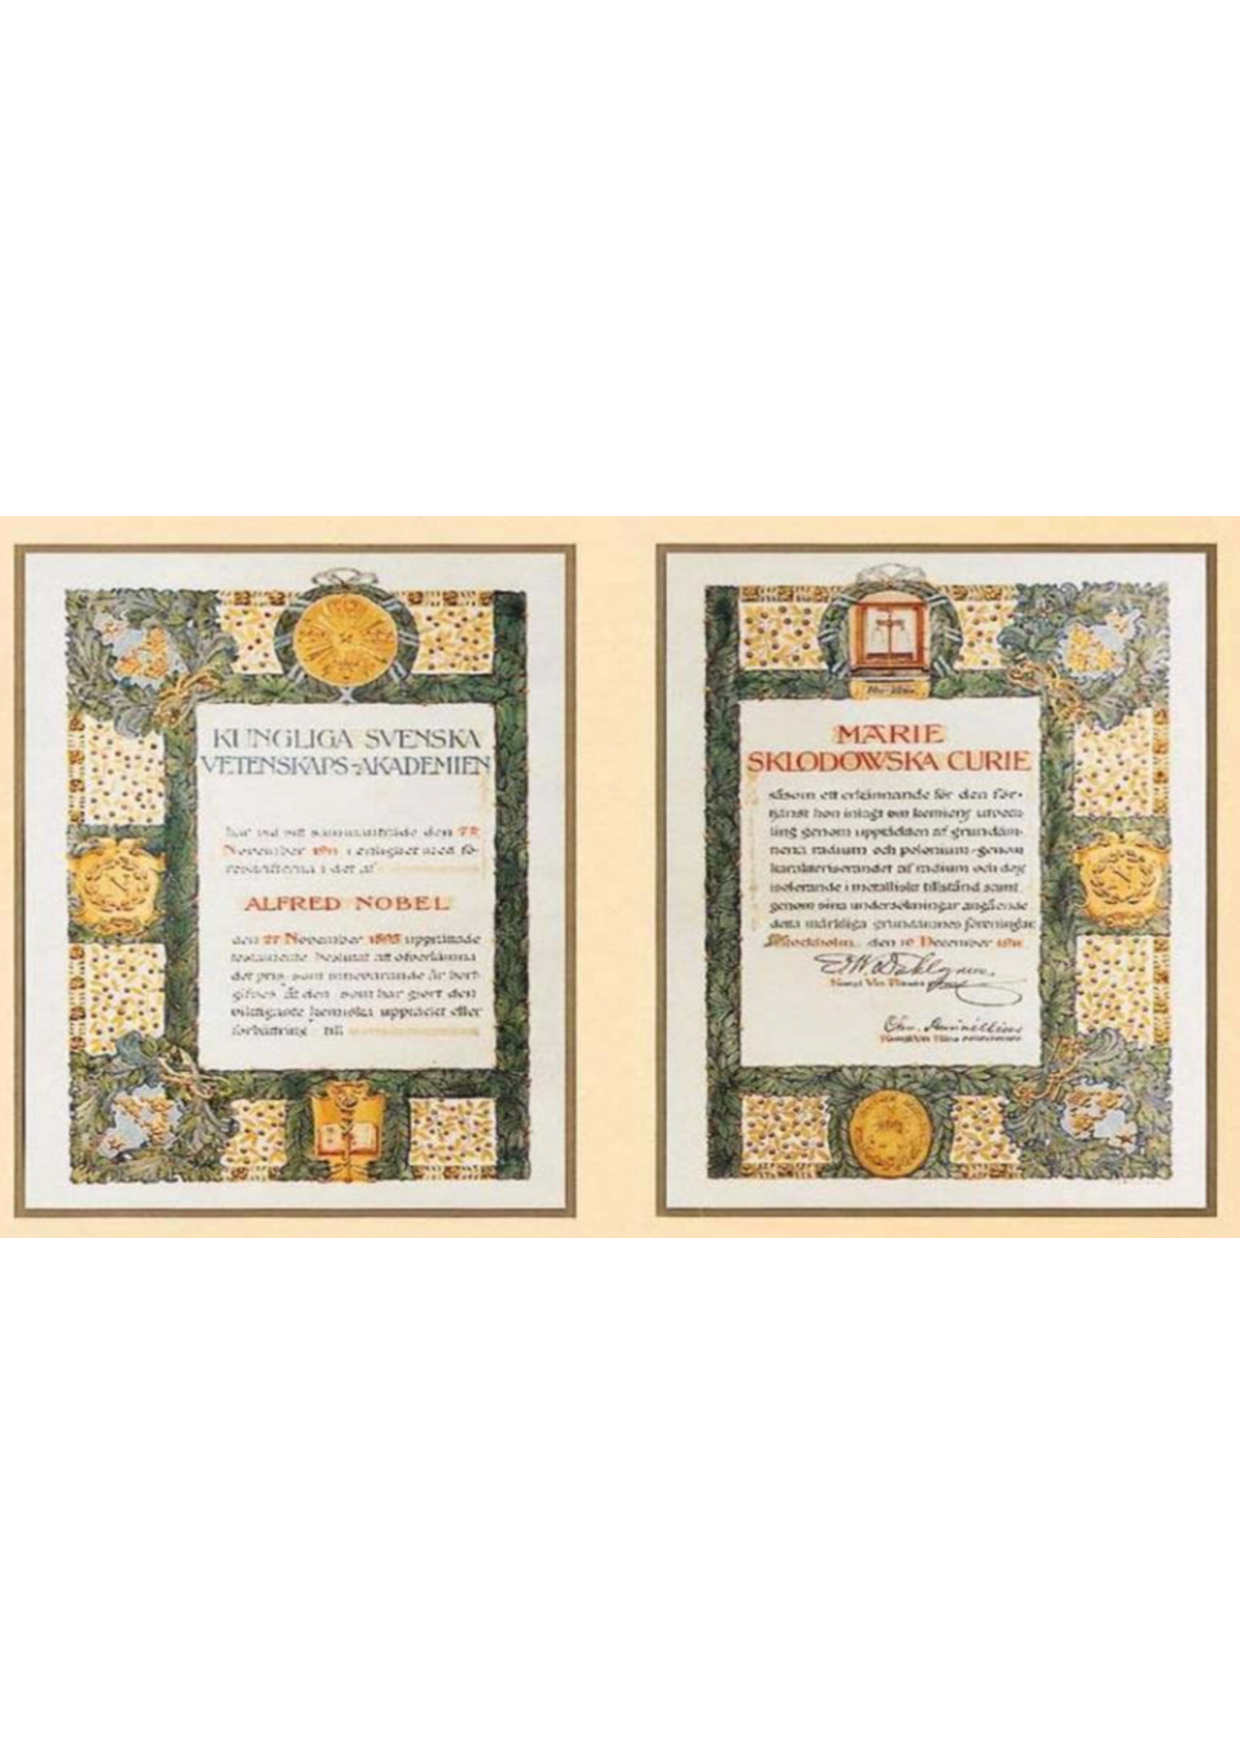
\includegraphics[scale=0.5]{figures/20160216_rsw_picnobel.pdf}
\end{frame}

\begin{frame}{Once upon a time \ldots}

  \begin{alertblock}{Other names to bear in mind}
    
\begin{columns}[T]

    \begin{column}{.4\textwidth}
     \begin{itemize}
     	\item Ernest Rutherford (1871 -- 1937): concept of radioactive half-life; model of the atom
     	\item Sir James Chadwick (1891 -- 1974): the discovery of the neutron
     	\item Frederick Soddy (1877 -- 1956): radioactivity and nuclear reactions
     \end{itemize}
    \end{column}
    
    \begin{column}{.4\textwidth}
\begin{itemize}
	\item Friedrich Ernst Dorn (1848 -- 1916): see later \ldots
	\item Rolf Maximilian Sievert (1896 -- 1966): biological effects of radiation
	\item Max Karl Ernst Ludwig Planck (1858 -- 1947): quantum theory
\end{itemize}    
    \end{column}

\end{columns}    
     \end{alertblock}

\end{frame}

\begin{frame}{Once upon a time \ldots}


\begin{figure}
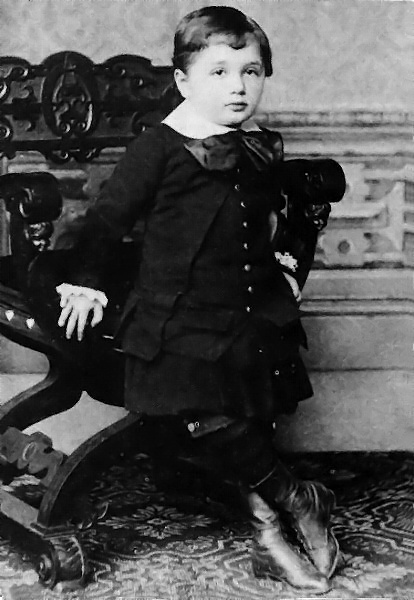
\includegraphics[scale=1]{figures/Albert_Einstein_3}
\caption*{\href{By YouTube - http://th.physik.uni-frankfurt.de/~jr/physpiceinstein.html., Public Domain, https://commons.wikimedia.org/w/index.php?curid=1821347}{\emph{Credit}}}
\end{figure}

\end{frame}

\begin{frame}{Once upon a time \ldots}

\begin{figure}
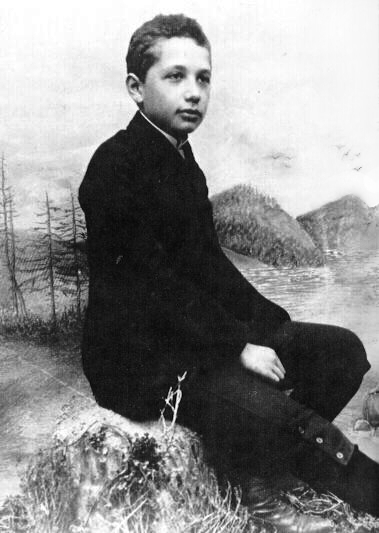
\includegraphics[scale=0.35]{figures/Albert_Einstein_child}
\caption*{\href{By Unknown - http://faculty.randolphcollege.edu/tmichalik/einstein.htm, Public Domain, https://commons.wikimedia.org/w/index.php?curid=3850884}{\emph{Credit}}}
\end{figure}

\end{frame}

\begin{frame}{Once upon a time \ldots}

\begin{figure}
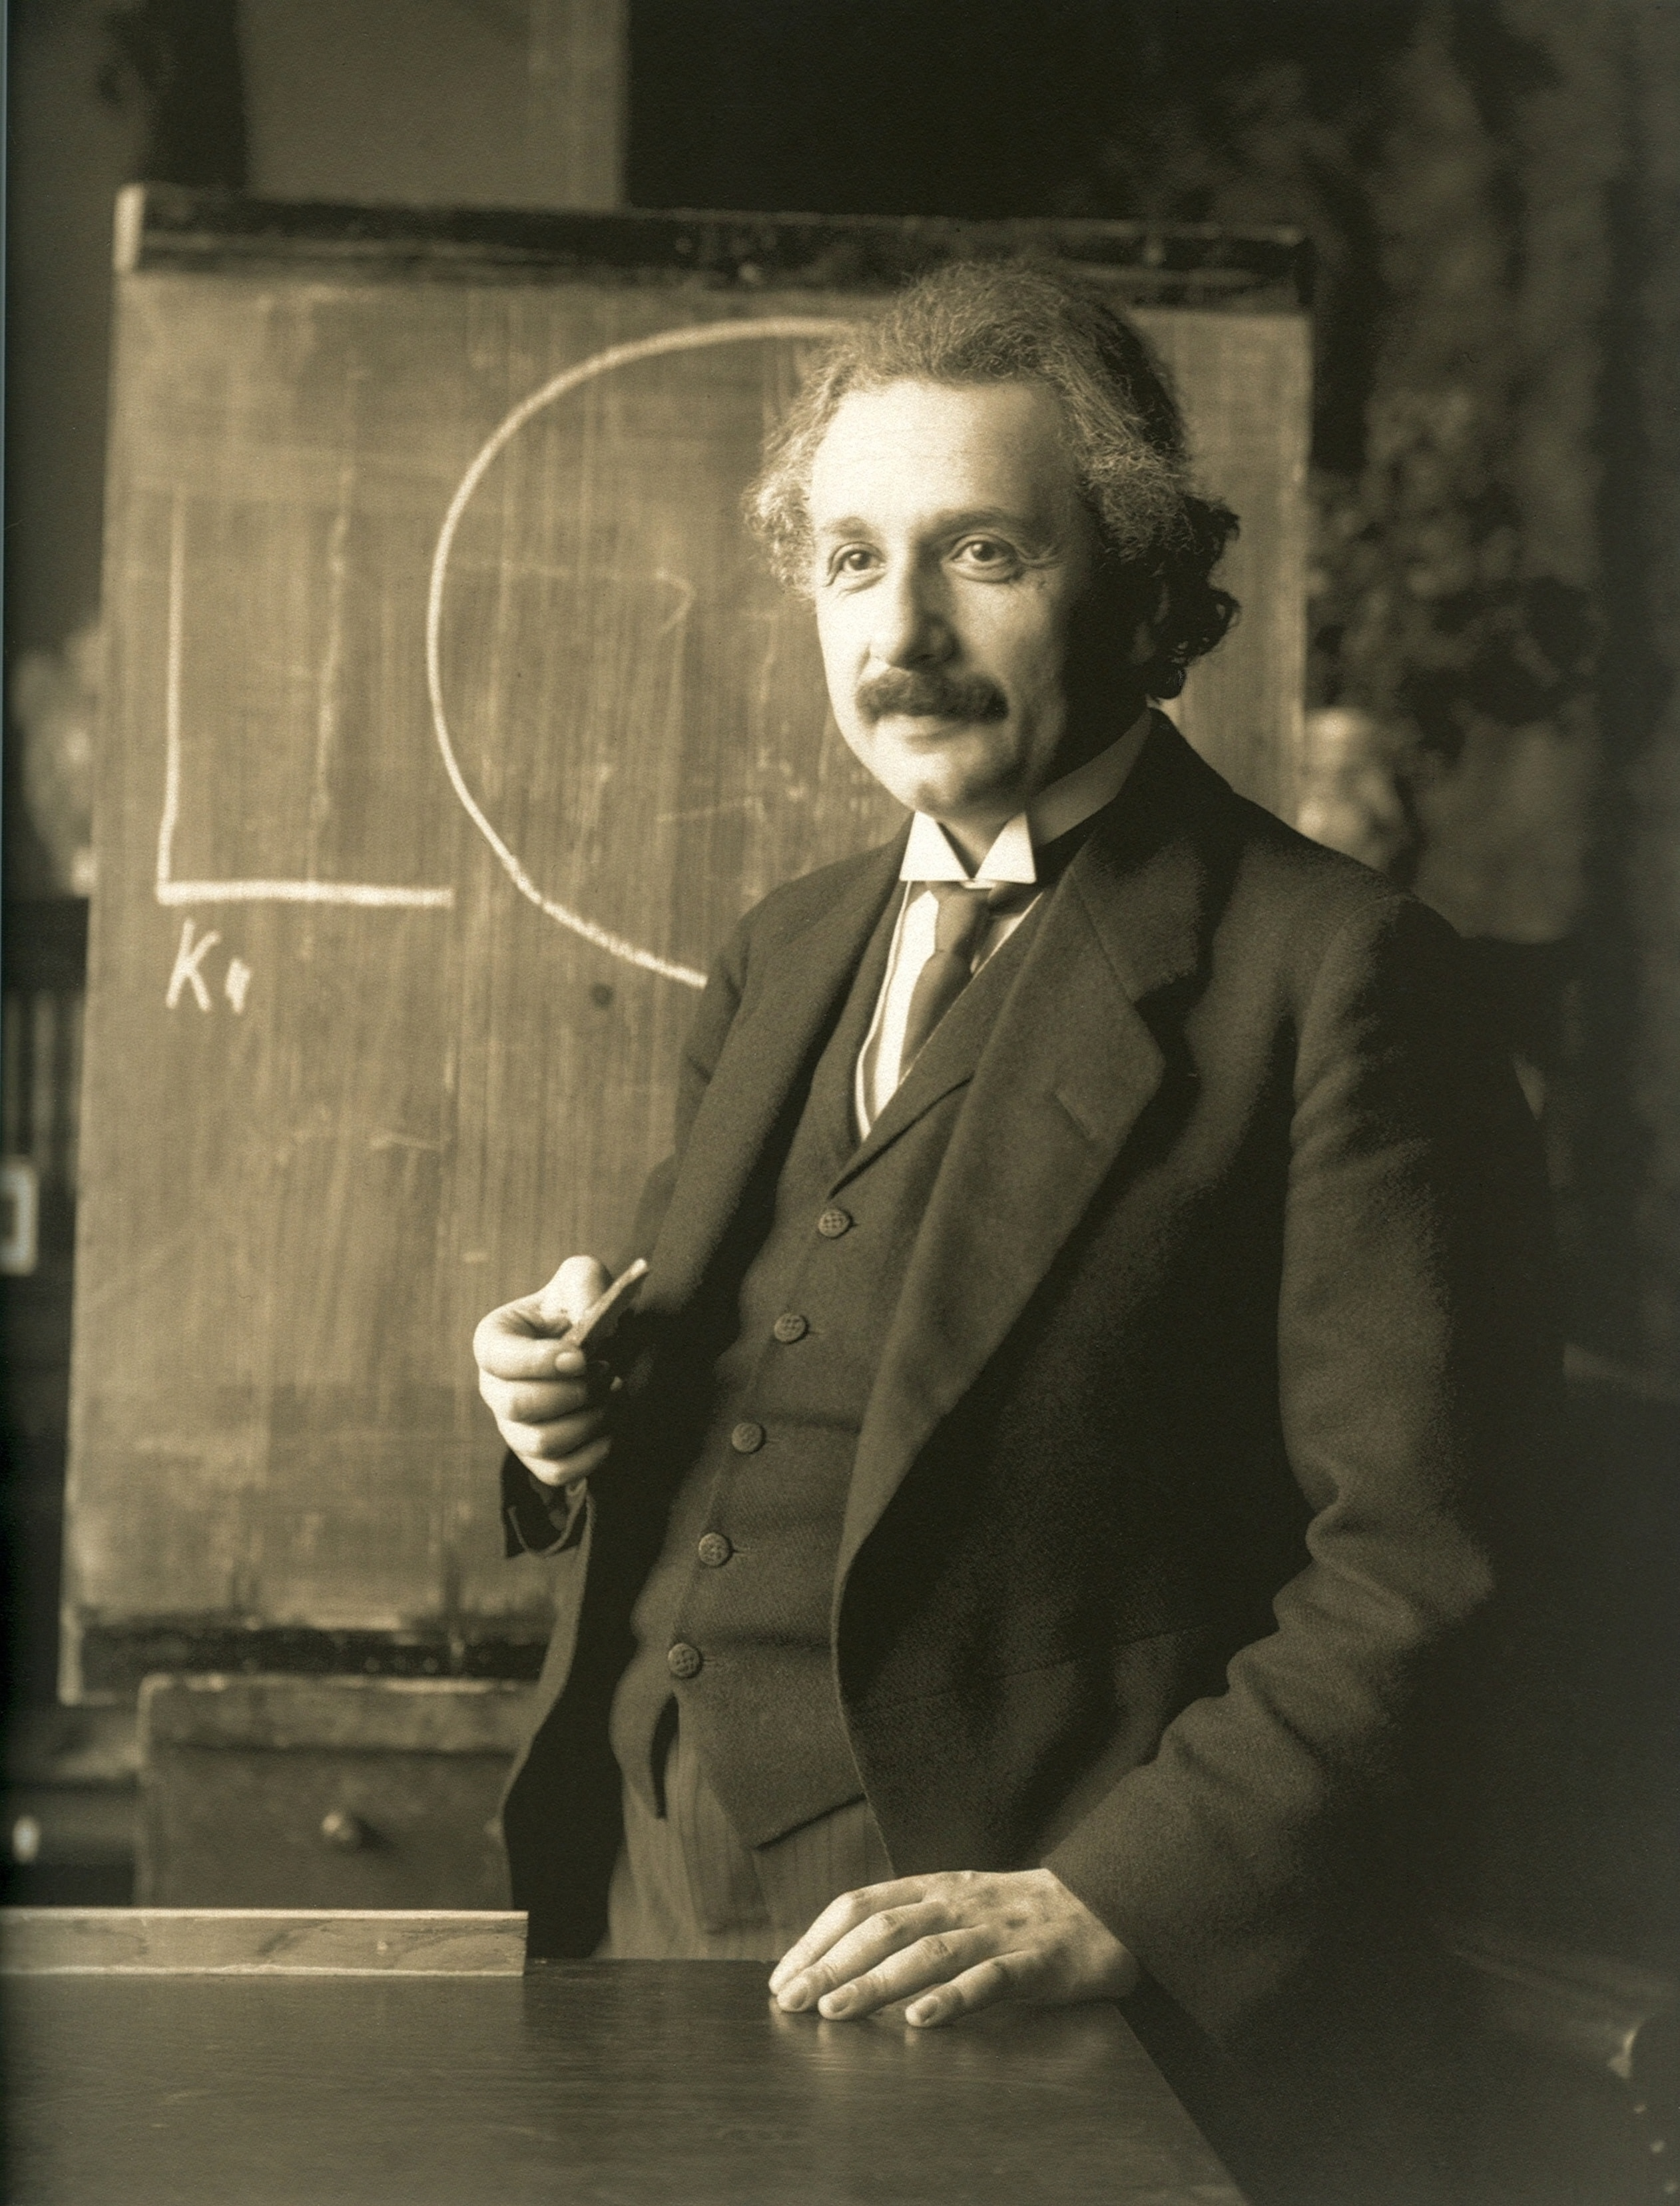
\includegraphics[scale=0.25]{figures/Einstein_1921}
\caption*{\href{By Ferdinand Schmutzer - http://www.bhm.ch/de/news_04a.cfm?bid=4&jahr=2006 [dead link], archived copy (image), Public Domain, https://commons.wikimedia.org/w/index.php?curid=34239518}{\emph{By Ferdinand Schmutzer}}}
\end{figure}

\end{frame}

\begin{frame}{Learnings so far}

\begin{alertblock}{Let's remember}

\begin{itemize}

\pause \item Radioactivity: new phenomenon discovered at the end XIX century

\pause \item Curie: key name on the development of knowledge XX century

\pause \item The beggining of XX century gathered a fantastic pool of scientist as ever

\end{itemize}

\end{alertblock}

\end{frame}

%\section{basics}
%
%\frame{\tableofcontents[currentsection]}
%
%\begin{frame}
%
%\end{frame}
%
%\section{conclusions}
%
%\begin{frame}
%
%\end{frame}

%-=-=-=-=-=-=-=-=-=-=-=-=-=-=-=-=-=-=-=-=-=-=-=-=
% ACKNOWLEDGEMENT SLIDE
%-=-=-=-=-=-=-=-=-=-=-=-=-=-=-=-=-=-=-=-=-=-=-=-=

%\begin{frame}{One minute paper}
%
%%\centering
%%\includegraphics[scale=0.4]{figures/20160126_rpw_cliffsmoher.jpg}
%
%\end{frame}



\section{Radioactivity: fundamentals}

\begin{frame}

\end{frame}


\end{document}


%
%  \begin{exampleblock}{Some more block}
%    Movies only seem to work in Adobe Reader\par
%    Movie file is not embedded, it must be on the computer
%  \end{exampleblock}
%
%  \begin{alertblock}{}
%    Some text in here.
%    \begin{itemize}
%    \item Movies only seem to work in Adobe Reader
%    \item Movie file is not embedded, it must be on the computer
%    \end{itemize}
%  \end{alertblock}
%\end{frame}



%\section
%  {Conclusion}
%
%\begin{frame}
%  {Credits}
%
%  \begin{itemize}
%  \item Brought to you by Cédric Mauclair
%  \item Please let me know about improvements!
%  \item inspiration: \url{http://www.shawnlankton.com}... (in code)
%  \end{itemize}
%\end{frame}


%\begin{frame}
%  {Questions}
%
%  \nocite{lorem,ipsum}
%  \bibliographystyle{plain}
%  \bibliography{demo}
%
%\end{frame}


